\documentclass[12pt ]{article} 
\usepackage{amssymb}
\usepackage{amsmath}
\usepackage{geometry}
\usepackage[slovene]{babel}
\usepackage[
sorting=none,
style=numeric,
sortcites=true]{biblatex}
\usepackage{import}
%\usepackage{tocbind}
%\usepackage[T1]{fontenc} 
\usepackage{float}
\usepackage{gensymb}
\usepackage{graphicx}
\usepackage{hyperref}
\usepackage{wrapfig}
\usepackage{siunitx}
\usepackage{caption}
\usepackage{pgfplots}

% externalize figures: create PDFs which are then imported into the document
\pgfplotsset{width=10cm}
\usepgfplotslibrary{external}
\tikzexternalize
\usetikzlibrary{arrows.meta}
\hypersetup{
  colorlinks,
  linkcolor={black},
  citecolor={black},
  %urlcolor={blue!80!black}
}
\geometry{a4paper,
 total={160mm,240mm}}
  
\newfloat{slika}{htbp}{loc}
\floatname{slika}{Slika}

\floatstyle{plaintop}
\newfloat{tabela}{htbp}{loc}
\floatname{tabela}{Tabela}

%\renewcommand{\baselinestretch}{0.9}

\addbibresource{refs.bib}
\DefineBibliographyStrings{slovene}{
  pagetotals = {strani}
}
 \begin{document}
 \pagenumbering{gobble}
 $~$ 
 
 \vspace{2cm}
 
 \centerline{\bf \huge   Mehurčne komore}
 
 \vspace{1cm}
 
  \centerline{\huge  Avtor: Kristofer Č. Povšič}
  
   \vspace{1cm}
  
  \centerline{\large Mentor: prof. dr. Simon Širca}
  
  \vspace{1cm}
  
  \centerline{\large Seminar, 3. letnik}
  
  \vspace{1cm}
  
  \centerline{\large Oddelek za fiziko, FMF, UL, 2025/2026}
  
  \vspace{6cm}
  
  \begin{minipage}[c]{0.9\hsize}
  {\bf Povzetek} V tem seminarju predstavimo dva modela, ki opisujeta nastanek mehurčkov v mehurčni komori, in si bolj podrobno ogledamo toplotni model. Opišemo načine iskanja šibko interagirajočih masivnih delcev. Predstavljena sta dva projekta, ki z mehurčnimi komorami iščeta dokaze o njihovem obstoju.
    \end{minipage}

 
 \newpage

 \pagenumbering{arabic}
 \tableofcontents
  
 \newpage

 \section{Uvod}\label{sec:uvod}

Izum mehurčne komore pripada Donald A. Glaserju, ki je leta 1952 odkril, da bo pregreta tekočina dietil etra pri temperaturi \( 130^{\degree} \mathrm{C} \) in tlaku 20 atmosfer vzkipnila ob prisotnosti \( ^{60}Co \)~\cite{glaser_effects_1952}. Za svoje izum je leta 1960 prejel Nobelovo nagrado. 

Mehurčne komore vsebujejo pregreto tekočino in, če vpadni delec pri sipanju odda dovolj energije elektronu, se pojavijo mehurčku in tekočina začne vreti~\cite{bressler_buffer-free_2019}. Fotoaparati z dovolj hitrim zajemanjem slik so lahko fotografirale sled mehurčkov, ki jih je za seboj puščal vpadni delec.

Po vretju tekočine se komori poviša tlak, plin se kondenzira, tlak se ponovno zniža in postopek se lahko ponovi~\cite{bressler_buffer-free_2019}. 

Na začetku so se mehurčne komore kot so Gargamelle in Velika evropska mehurčna komora\ (ang. \textit{Big European Bubble Chamber} ali BEBC) uporabljale za sledenje delcem v trkih z visokoenergijskimi delci\cite{noauthor_archives_nodate}. Komore so bile obdane s superprevodnimi magneti, ki so lahko proizvedli magnetno polje do \( 3.5 \mathrm{T} \)~\cite{\BEBC}. Nabiti delci so se, odvisno od predznaka naboja

 \section{Delovanje mehurčne komore}

Izumitelj mehurčne komore, D. A. Glaser, je predpostavil, da je za nastanek mehurčkov kriva elektrostatska sila med električnimi naboji, ki jih povzroči ioniziran delec\cite{glaser_bubble_1958}. Glaser je sčasoma opustil svojo teorijo\cite{seitz_theory_1958}. V seminarju bom predstavil dve od možnih teorij, kako nastanejo mehurčki v mehurčni komori. Zaradi narave uporabe mehurčne komore, tj. visokoenergijske raziskave, fokus nikoli ni bil na njenem delovanju, ampak na možnih novih spoznanjih kot posledica raziskav\cite{seitz_theory_1958}. Prva teorija predstavi termalni model, ki ga je oblikoval Seitz, in predpostavlja nastanek ``termalni skokov'' (ang. \textit{thermal spikes})\cite{seitz_theory_1958}. Druga teorija je novejša, iz leta 1998, in nastanek mehurčkov v vodikovih in helijevih komorah pripisuje mehanskemu procesu\cite{konstantinov_how_1998}. Seitzov model je trenutno sprejet kot najboljša razlaga nukleacije mehurčkov kot posledice sevanja v pregretih tekočinah\cite{bruno_critical_2019}.

\subsection{Termalni model}

Komora je napolnjena s pregreto kapljevino kot so helij, devterij, vodik, propan, freon ali ksenon\footnote{Glaser je v komunikaciji s Seitzom predstavil dokaze, da zelo čist(?) ksenon ni občutljiv na sevanje, vendar postane ob dodajanju malih količin etilena.}. Spomnimo, da je pregreta kapljevina kapljevina, ki smo jo počasi segreli nad njeno vrelišče pri konstantnem tlaku, brez da bi kapljevina zavrela. To lahko storimo, če je stena posode gladka, kapljevina miruje in v njej ni drugih delcev\cite{strnad_fizika_2016}. Metastabilno stanje pregrete kapljevine se popravi v stabilno v trenutku, ko nastane v njej mehurček, kapljevina pa eksplozivno vzkipi. Temperatura kapljevine pade na vrelišče.



\subsection{Mehanski model}


 \section{Detekcija temne snovi}

Če se ponoči zazremo v nebo, vidimo neskončno mnogo svetlih objektov, vendar je celotne vidne mase v vesolju zgolj \( 15 \% \), preostanek pa jo sestavlja temna snov, ki se deli na barionsko in nebarionsko. Bralca spomnimo, da je barionska snov sestavljena iz barionov kot so protoni in nevtroni. Trenutni rezultati eksperimentov kažejo, da je večino temne snovi nebarionske. Temno snov delimo na dva razreda -\` masivne astrofizikalne objekte v haloju (ang. \textit{massive astrophysical compact halo object} ali MACHO)~\cite{jones_introduction_2004} in hipotetične masivne delce s šibko interakcijo (ang. \textit{Weakly Interacting Massive Particles} ali WIMP)~\cite{noauthor_delec_2026}.

Kratka teorije glede WIMP-ov je povzeta iz vira~\cite{feng_dark_2010}. Njihova napovedana masa je v območju \( m_{weak} \sim 10 \, \mathrm{GeV} - \mathrm{TeV} \) in kakor pove ime interagirajo z drugimi delci preko šibke interakcije z bozonoma \( W \) in \( Z \). Po teoriji Velikega poka je bilo zgodnje vesolje gosto in vroče in delci so bili v stabilnem stanju. Ko se je vesolje kasneje ohlajalo, je temperatura \( T \) padla pod maso delca temne snovi. Boltzmannova porazdelitev nam pove verjetnost, da ima sistem določeno energijo\cite{noauthor_boltzmann_nodate}. Zaradi nje so temni delci postali zavrti in eksponentno padali \( \exp \left\{ - m_X / T  \right\} \). V naslednjem koraku se je vesolje tudi širilo, kar pomeni, da so bili delci temne snovi tako redki, da je bila njihove medsebojna anihilacija nemogoča. Število temnih delcev se tako asimptotsko približuje konstantemu številu.

WIMP-i \( X \) se torej morajo anihilirati z drugimi delci in pod predpostavko, da so te delci \( \mathrm{SM} \) del standardnega modela, potem mora obstajati interakcija \( X \, X \to \mathrm{SM} \, \mathrm{SM} \). To nam poda tri možne načine zaznave temne snovi. Če drži, da so se \( X \) anihilirali v zgodnjem vesolju, potem se morajo tudi sedaj \( X \, X \to \mathrm{SM} \, \mathrm{SM} \) in zaznamo lahko ostanke anihilacije. Temu načinu pravimo nedirektna detekcija. V trkalnikih delcev je temna snov lahko rezultat trka \( \mathrm{SM} \, \mathrm{SM} \to X \, X + \{SM\} \) in zaznamo produkte, ki nastanejo poleg temne snovi.

Zadnja vrsta detekcije, ki se tiče tega seminarja, je direktna. Temna snov se lahko sipa na normalni snovi preko interakcije

\begin{equation}
\label{eq5:1}
 X \, \mathrm{SM} \to X \, \mathrm{SM},
\end{equation}

in s tem odda svojo energijo.

Sipanje je odvisno od lokalne gostote toka \( X \) in sipalnega preseka za interakcijo. Fiksna lokalna gostota delcev \( X \) pa je odvisna od njihove mase. Eksperimentalna spremenljivka je zato izražena kot masa WIMP-a v odvisnosti od sipalnega preseka. Slednji je odvisen od interakcije WIMP-nukleon in ga delimo na spinsko odvisno in spinsko neodvisno WIMP-nukleon interakcijo~\cite{collaboration_moscab_2017}. 

Sipalni presek spinsko odvisnih interakcij je odvisen od jedrskega spinskega števila. Opisana projekta oba uporabljata na floru bazirane tekočine v mehurčni komori, saj ima jedro flora \( ^{19}F \) en nepoparjen proton, hkrati pa nima izotopov~\cite{ellis_realistic_1988}. Take tekočine imajo torej edinstveno prednost.

Mehurčne komore so dobri detektorji za direktno iskanje WIMP-ov, saj so neobčutljivi na \( \beta \) in \( \gamma \) sevanje, saj se nahajajo globoko v Zemlji\cite{collaboration_moscab_2017}. Dober detektor bo imel torej tarčo s čim večjo maso, hkrati pa bo bil občutljiv na energije pri sipanju v velikosti \( 1 - 100 \mathrm{keV} \)~\cite{amole_dark_2019}.

PICO je eden od projektov, ki preko direktne zaznave iščejo dokaze o temni snovi. Je del podzemnega laboratorija SNOLAB, ki se nahaja v Sudbury, Ontaorio v Kanadi. Od svojega nastanka 2013, ko sta se združila projekta PICASSO laboratorija SNOLAB in COUPP laboratorija Fermilab, je potekala že vrsta eksperimentov PICO-2, PICO-40 in PICO-60, kjer številka izraža količino freona v mehurčni komori. V pripravah je PICO-500\cite{noauthor_pico_nodate}. 

\begin{wrapfigure}{r}{8cm}
  \begin{center}
  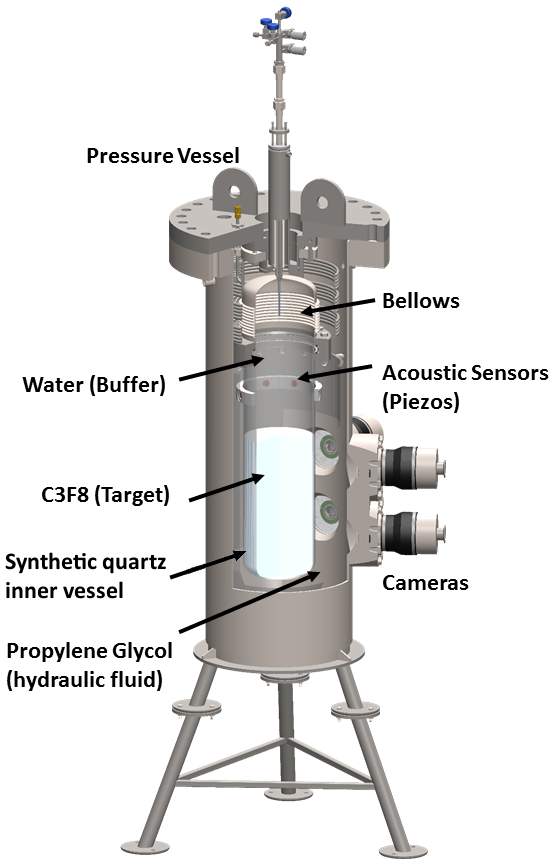
\includegraphics[width=0.25\textwidth]{./figures/PICO60Run2_IV_label}
  \end{center}
  \caption{\small Detektor PICO60~\cite{amole_dark_2019}}
\end{wrapfigure}

PICO mehurčna komora je precej drugačna od 



 \section{Zaključek}

Spoznali smo kratko zgodovino mehurčnih komor dva teoretična modela delovanje mehurčne komore -\ toplotnega in mehanskega. Izpeljali smo enačbo za energijo stabilnega mehurčka in jo primerjali z energijo, ki jo sipan delec odda elektronu. Rast mehurčka do makroskopske velikosti je odvisna tudi od viskoznosti tekočine.

Opisani so bili načini iskanja WIMP-ov ter dva izmed projektov, kjer iščejo dokaze o njihovem obstoju.

 \newpage
 \printbibliography[heading=bibintoc,
 title=Bibliografija]

\end{document} 
